\documentclass[9pt,twocolumn,twoside]{opticajnl}
\journal{opticajournal} % use for journal or Optica Open submissions

% See template introduction for guidance on setting shortarticle option
\setboolean{shortarticle}{false}
% true = letter/tutorial
% false = research/review article

% ONLY applicable for journal submission shortarticle types:
% When \setboolean{shortarticle}{true}
% then \setboolean{memo}{true} will print "Memorandum" on title page header
% Otherwise header will remain as "Letter"
% \setboolean{memo}{true}

\usepackage{lineno}
\usepackage[inkscapeformat=png]{svg}

\linenumbers % Turn off line numbering for Optica Open preprint submissions.

\title{Training and Validation of Moment Tensor Potentials for Potassium Metal}

\author[1,2,3]{ Richard Meng}
\author[1]{Laurent  Béland}
\author[1]{Hao Sun}

\affil[1]{Department of Mechanical and Materials Engineering, Queen's University, 45 Union St, Kingston, ON K7L 3N6}

\affil[2]{contact@richardzjm.com}
\affil[3]{17zjm1@queensu.ca}

\begin{abstract}
This template can be used to approximate final page count for submission to Optica Publishing Group’s journals \emph{Applied Optics}, \emph{Journal of Optical Communications and Networking}, JOSA A, JOSA B, \emph{Optics Letters}, \emph{Optica}, and \emph{Photonics Research}. Use the shortarticle/true option for \emph{Optics Letters} and short \emph{Optica} articles.  Authors may also \href{https://opticaopen.org}{submit articles} prepared using this template to the Optica Publishing Group preprint server, \href{https://preprints.opticaopen.org}{Optica Open}. However, doing so is optional. Please refer to the submission guidelines found there. Note that copyright and licensing information should no longer be added to your Journal or Optica Open manuscript.
\end{abstract}

\setboolean{displaycopyright}{false}
\doi{\url{https://www.richardzjm.com/projects} \\ \url{https://github.com/RichardZJM/K-MTP-training}}

\begin{document}

\maketitle

\section{Introduction}
Molecular Dynamics (MD) has been an invaluable tool in fields such as computational chemistry, materials science, and pharmaceutical drug discovery, for modelling the motions of atoms and predicting the properties of compounds \cite{karplus2002molecular}. MD models atomic motions using a classical representation of atoms, representing them as particles and applying the interatomic forces to numerically solve the equations of motion.

Quantum chemistry methods provide perhaps the best descriptor of the interatomic methods. With considerations for the electrons of the system, techniques like Density Functional Theory (DFT) and Hartree-Fock methods provide a high-fidelity force calculation by approximating a solution to the many-bodied Schrödinger Equation \cite{DFT}. However, this comes with a cubic time complexity and considerable expense even for a system of moderate size.  A single timestep in a DFT MD run of 56 atoms took several hours on 48 cores. 

Interatomic potentials, less expensive descriptors which approximate interatomic forces predictions, are usually used. In the simplest case, pair potentials such as the Lennard-Jones Potential or the Morse Potential can be used to describe the forces between all pairs of atoms with a simple function of pair-wise separation. More sophisticated many-body potentials like EAM potentials for metals and the bond order potentials for covalent solids have seen widespread practical use \cite{MatSci}. Much of recent research in interatomic potential development has been focused on machine learning (ML) potentials. These offer an improvable and adaptable approach to force modelling which is more made accessible by the relative ease of training data acquisition through quantum modelling methods. Some of the common categories of ML potentials include neural networks, Gaussian approximation potentials, and linear regression on basis sets \cite{mlip}.

The Moment Tensor Potential (MTP) falls into this last category, making considerations for the radial and angular interactions. These contributions are evaluated within a cutoff radius, taking the sum of learnable linear combinations on the atom-atom positions \cite{mtp}. The MTP architecture can be enhanced with an active learning scheme, applying the D-optimality criterion on the information matrix formed by the value of the basis functions for a set of configurations. Thus, an MTP can decide whether newly encountered configurations will be likely misrepresented or are worthwhile to learn from, selecting them on the fly for further training through DFT calculations.

\section{MTP Architecture}
We provide a brief overview of the linearly-parameterized MTP architecture. More rigorous explanations are available from the source paper \cite{mtp}.

In the MTP, the total energy of a configuration, $E^{MTP} (\textrm{cfg}) $, is represented by the total contributions, $V(n_i)$, of the local environment of each atom, shown in Equation \ref{eq:configEnergy}.  $V(n_i)$ is represented by the relative positions of atoms within a cutoff radius of the $i$th atom.

\begin{equation} \label{eq:configEnergy}
  E^{MTP} (\textrm{cfg}) = \sum_{i=1}^{n} V(n_i)
\end{equation}

For each atom, the contribution is a linear combination of a set of learnable weights, $\xi = \{\xi_\alpha\}$ and the basis set, shown in Equation \ref{eq:basisSet}.

\begin{equation} \label{eq:basisSet}
  V(n_i) = \sum_{\alpha} \xi_\alpha   B_\alpha (n_i)
\end{equation}

The elements of this basis set are formed from but not necessarily directly formed from moment tensor descriptors or simply \textit{moments}. A moment, $M_{\mu,\nu}$,  is characterized by a $\mu$ and a $\nu$ value, and has level, $\textrm{lev}_{max}$, which is given by \ref{eq:levelMTP}.

\begin{equation} \label{eq:levelMTP}
  \textrm{lev}M_{\mu,\nu} = 2 + 4\mu + \nu
\end{equation}

Each moment, given by Equation \ref{eq:moment}, has a radial part, $f_\mu (|r_{ij}|,z_i,z_j) $, characterized by the moment's $\mu$ value,  based on the distance between atoms, $|r_{ij}|$, and the species, $z_i$ and $z_j$. It also has an angular part, given by $r_{ij} ^{\otimes \nu}$.

\begin{equation} \label{eq:moment}
  M_{\mu,\nu} (n_i)= \sum_{j} f_\mu (|r_{ij}|,z_i,z_j) r_{ij} ^{\otimes \nu}
\end{equation}

\subsection{Radial Considerations}
The radial component, given by Equation \ref{eq:radial}, expands into a linear combination of a set of learnable weights $c = \{c^{(\beta)} _ {\mu,z_i,z_j} \}$, on a basis set of radial functions.

\begin{equation} \label{eq:radial}
  f_\mu (|r_{ij}|,z_i,z_j) = \sum ^ {N_o} _ {\beta = 1} c^{(\beta)} _ {\mu,z_i,z_j}  Q^{(\beta)}(|r_{ij}|)
\end{equation}

The radial functions, given in Equation \ref{eq:cheby}, are simply members of a polynomial basis set, usually Chebyshev polynomials of the first order, $\phi$, which are quadratically smoothed towards the cutoff radius, $R_{\textrm{cut}}$, to preserve a continuous second derivative.

\begin{equation} \label{eq:cheby}
  Q^{(\beta)}(|r_{ij}|)=  \begin{cases}
    \phi ^{(\beta)}(|r_{ij}|) (R_{\textrm{cut}} - |r_{ij}|)^2& |r_{ij}| < R_{\textrm{cut}} \\
    0 & |r_{ij}| \geq R_{\textrm{cut}} 
\end{cases}
\end{equation}

\subsection{Angular Considerations}
The angular component, $r_{ij} ^{\otimes \nu}$, represents the outer product of $\nu$ copies of the relative position vectors between atoms $i$ and $j$. This yields a tensor of dimension equal to $\nu$. These values are not scalars, although they could yield scalars on their contraction.

\subsection{Contraction of Tensors}
Since the contribution is reliant on a linear combination of the basis functions, moments cannot directly be applied to form the basis functions due to the tensors possibly having different ranks. Instead, contractions are performed on some number of moments, which can ultimately lead to a scalar value. Much like moments have levels, the level of a contraction of moments is the sum of the levels of the constituent moments.

When choosing the hyperparameters of an MTP, we define a maximum level, $\textrm{lev}_max$, and take all contractions of moment tensor descriptors which have a level less than or equal to this maximum level. Two other key hyperparameters in the MTP model are the cutoff radii (lower and upper bound) and the number of elements in the basis set.

\section{Active Learning}
The MTP is also capable of active learning, which allows the MTP to evaluate new configurations it encounters in use. When given a set of training configurations, each training configuration will produce a set of basis functions for each atom \cite{mlip}. These per-atom basis function values can be summed up to generate a per-configuration value of each basis function.

\begin{equation}
  E^{MTP}(\textrm{cfg}) = \sum_i \sum_\alpha^m \xi_\alpha B_\alpha (n_i) = \sum_\alpha^m \xi_\alpha (\sum_i  B_\alpha (n_i)) = \sum_\alpha^m \xi_\alpha b_\alpha
\end{equation}

Thus, for each training configuration, we can formulate a vector of the per-configuration value of the basis functions, $b(\textrm{cfg})$. Taking these vectors of rows, we can form a matrix with a height equal to the number of training configurations and a width equal to the number of basis functions in the chosen level of MTP.  For $n$ training configurations with $m$ basis functions we have that,

\[
\begin{bmatrix} 
    b_{1}(\textrm{cfg}_1)  & b_{1}(\textrm{cfg}_2)  & \cdots & b_{\alpha}(\textrm{cfg}_1) \\
    b_{2}(\textrm{cfg}_2)  & b_{2}(\textrm{cfg}_2)  & \cdots & b_{\alpha}(\textrm{cfg}_2) \\
    \vdots & \vdots & \ddots & \vdots \\ 
    b_{1}(\textrm{cfg}_n)       & b_{2}(\textrm{cfg}_n)  & \dots & b_{\alpha}(\textrm{cfg}_n) 
\end{bmatrix}
\]


In cases where there are more training configurations than we have basis functions, $m < n$, this matrix would be tall. Applying the D-optimality criterion, the $m$ rows which compose the $m$ by $m$ square submatrix, $A$, that has the largest determinant magnitude are taken to be the most linearly independent members of the training set. When the MTP is used in an MD simulation, it can assess whether a newly encountered configuration, $\textrm{cfg}_x$ would increase the magnitude of $A$'s determinant. MTP evaluates $c_i(\textrm{cfg}_x)$, the degree to which the determinant would be changed should the new configuration $x$ replace the $i$th member of the current submatrix $A$, using \ref{eq:actLearn}.

\begin{equation} \label{eq:actLearn}
  c(\textrm{cfg}_x)  = (c_1(\textrm{cfg}_x) \cdots c_m(\textrm{cfg}_x)) = (b_1(\textrm{cfg}_x) \cdots b_m(\textrm{cfg}_x)) A^{-1}
\end{equation}

The extrapolation grade is then defined at the maximum possible change in the magnitude of the determinant of $A$, This is equivalent to the maximum of the vector $c(\textrm{cfg}_x)$.

\begin{equation}
  \gamma(\textrm{cfg}_x) = \max c_1(\textrm{cfg}_x)
\end{equation}

Should the extrapolation grade be below 1, the newly encountered configuration is conceptually interpolating relative to the existing database. Grades above 1 correspond to interpolation or a new configuration. Interpolation would imply that adding the new configuration would allow the training set to encompass a richer (more linearly independent) representation, providing an evaluation criterion for determining future training on the fly. When a new configuration is added, it replaces the corresponding member in the submatrix $A$.

\section{Objectives}
As an interatomic potential of interest to the Queen's Nuclear Materials Group, we look to explore the behaviour and validity of the MTP for Potassium metal. Precisely we aim to:
\begin{itemize}
  \itemsep0em
  \item Train general-purpose MTPs of potassium metal for temperature ranges which span the solid and liquid phases, under reasonable levels of pressure and strain. 
  \item Explore the effects of various MD learning simulations and training schemes on the active learning of an MTP.
  \item  Test the sensitivity of the MTP to hyperparameters and the initial, randomized learnable parameters. 
  \item Validate the MTP with physical property prediction against DFT results: elastic properties, radial distribution function (RDF), and configuration errors.
\end{itemize}


\section{Methodology}

\subsection{Simulation Software and Hardware}
To perform DFT calculations, we utilize the Quantum Esperso PWF code \cite{QE}. Molecular Dynamics are performed using LAMMPS  \cite{LAMMPS}. The MTPs being trained are available from the MLIP package which can be complied with a LAMMPS interface \cite{mlip}. We perform the calculation on the Digital Research Alliance of Canada Narval Cluster and the Queen's University Frontenac Cluster. Most simulations are performed on a single core with some of the more intensive calculations performed on 24 or 48 cores. 

\subsection{DFT Parameters and Base Lattice Parameter}
To produce generally applicable MTPs, and examine the practical applicability of the MTP, we emphasize the importance of a \textit{representative} training scheme for the target phases and environments. To examine potassium metal in reasonable solid and liquid phases, we target performance within 100-1000K, with minor strains and pressures.

DFT calculations are performed using the Quantum Espresso pseudopotential \cite{DFT}. We start by performing convergence testing for the k-point count (8 for a single BCC lattice) and the plane-wave cutoff values (60 Ry). Using, a range of DFT calculations, we arrive at a predicted lattice parameter of 5.11 Å. Future training and simulations were based on these baseline values. 

\subsection{Training of MTPs}
Before subjecting MTPs to MD runs to train through active learning, we initially train the MTP on a sufficient amount of configurations to provide a base representation of the behaviour. We settled on a range of single-atom configurations of BCC potassium under triaxial strain, $[0.75, 1.25]$; single-atom configurations under shear strain, $[0, 0.785]$; and two-atom configurations under triaxial strain $[0.9, 1.1]$. 

After the initial training, we subject the MTPs to a bottom-up training scheme in which we introduce the MTP to parallel MD simulations of BCC lattice cells under a range of conditions (pressures and temperatures) for a simulation cell size. When an MTP is \textit{}{sufficiently trained} a simulation cell size, we expose it to the subsequent simulation size in the training scheme. The rationale behind such an approach is to capture most of the interactions between potassium atoms at lower simulation cell sizes, and thus reduce the amount of overall computation required, especially considering the non-linear scaling of DFT.  Furthermore, we wish to limit the rate at which the MTP learns, for fear that learning from excessively extrapolative configurations may cause the number of training configurations not within the submatrix $A$ to become excessively sparse. 

  We define \textit{}{sufficiently trained} using the criteria proposed by the MLIP package \cite{mlip}. Using the extrapolation grade, we use preselect configurations with values in the range $[2, 10)$ for further training, and take grades larger than 10 as risky configurations, terminating the active MD run and initiating the retraining of the MTP. In the retraining, preselected configurations that are too similar are removed, generating the selected configurations for which DFT calculations are performed and expanding the training set. A diagram of this scheme is shown in Figure \ref{fig:extrapolation}.

  \begin{figure}[ht]
    \centering
    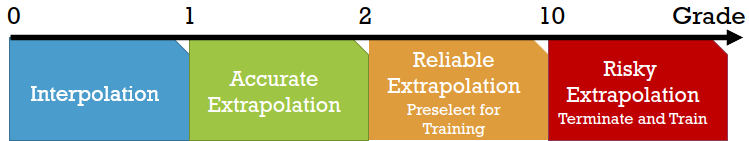
\includegraphics[width=\linewidth]{assets/grade.png}
    \caption{Configuration categorization based on extrapolation grade}
    \label{fig:extrapolation}
  \end{figure}

  We take an MTP to be \textit{sufficiently trained} relative to a simulation cell size when all the parallel MD runs return no preselected configurations. We take an MTP to have completed learning when it has passed through all of the simulation cell sizes in the scheme.

  In the bottom-up training approach, we choose six simulation cell sizes, shown in Table \ref{tab:stages}. Each stage consists of BCC unit cells of potassium. In the parallel MD runs, the dimensions of these are modified by the applied strains. The final scheme was chosen through experimentation as $3\times 3\times 3$ tended to produce no preselected configurations at all.

\begin{table}[htbp]
  \centering
  \caption{\bf Training Scheme Stages}
  \begin{tabular}{cccc}
  \hline
  Stage & $X$ count & $Y$ count & $Z$ count\\
  \hline
  1 & 1 & 1 & 1\\
  2 & 1 & 1 & 2\\
  3 & 1 & 1 & 3\\
  4 & 1 & 2 & 2\\
  5 & 2 & 2 & 2\\
  6 & 3 & 3 & 3\\
  \hline
  \end{tabular}
  \label{tab:stages}
\end{table}

Overall, the complete training of the MTPs can be summarized by the flowchart in \ref{fig:scheme}. For each of the stages, we perform 24 parallel MD runs under six strains in the range of ${0.95, 1.05}$ and four temperatures, 100 K, 330K, 400K, 800 K. This scheme aims to generate training datasets that model solid and liquid configurations, including temperatures near the empirical potassium melting point. These MTP runs are initiated from a perfect BCC lattice structure, before simulating under a Langvin $NVT$, in the hope of easing the number of risky configurations encountered for liquid modelling and sampling configurations near coexistence. Each MTP uses a first-order Chebyshev polynomial basis set with 8 members, and a cutoff radius of 8 Å. Experimentation with these values yielded no substanstial benefit with higher values beyond this point.  

\begin{figure}[ht]
  \centering
  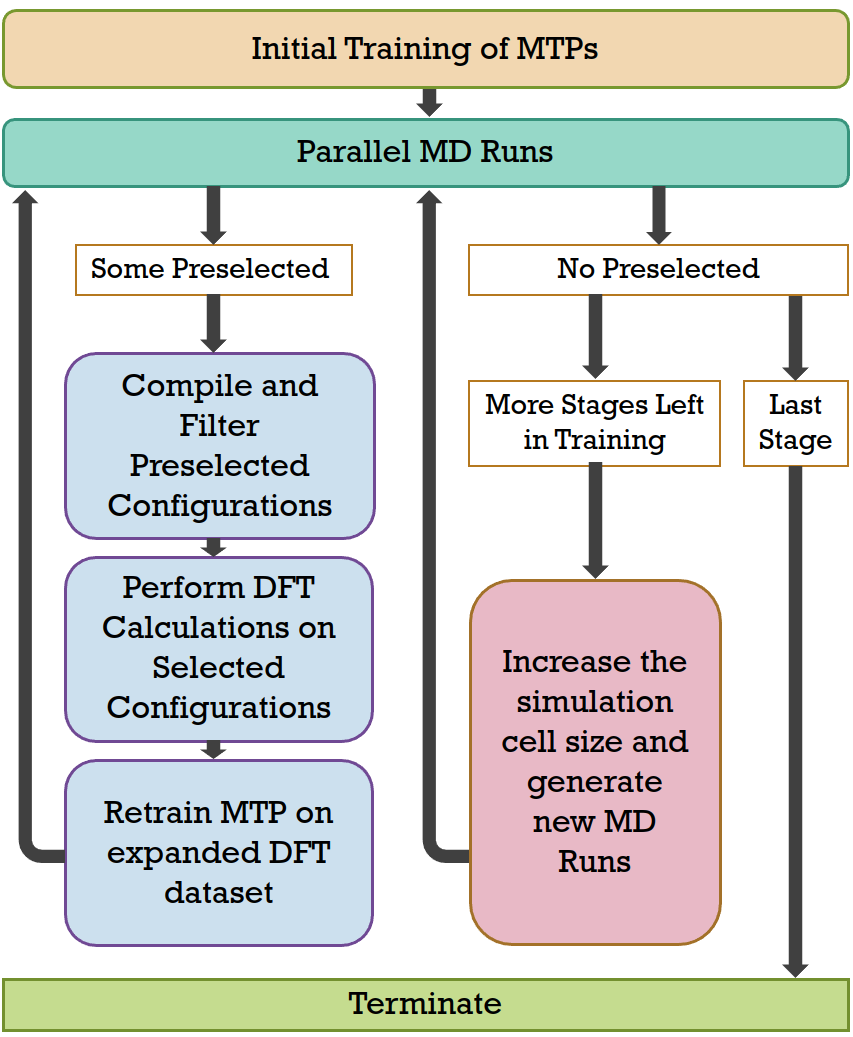
\includegraphics[width=\linewidth]{assets/trainingScheme.png}
  \caption{Configuration categorization based on extrapolation grade}
  \label{fig:scheme}
\end{figure}


\section{Results and Discussion}
To gauge the effectiveness of the MTPs of different levels and assess the validity of the bottom-up training scheme, active learning runs were performed using even MTP levels from 6 to 14. Figure \ref{fig:iterations} displays the percentage of the total iterations during each stage of the active learning runs. 

\begin{figure}[ht]
  \centering
  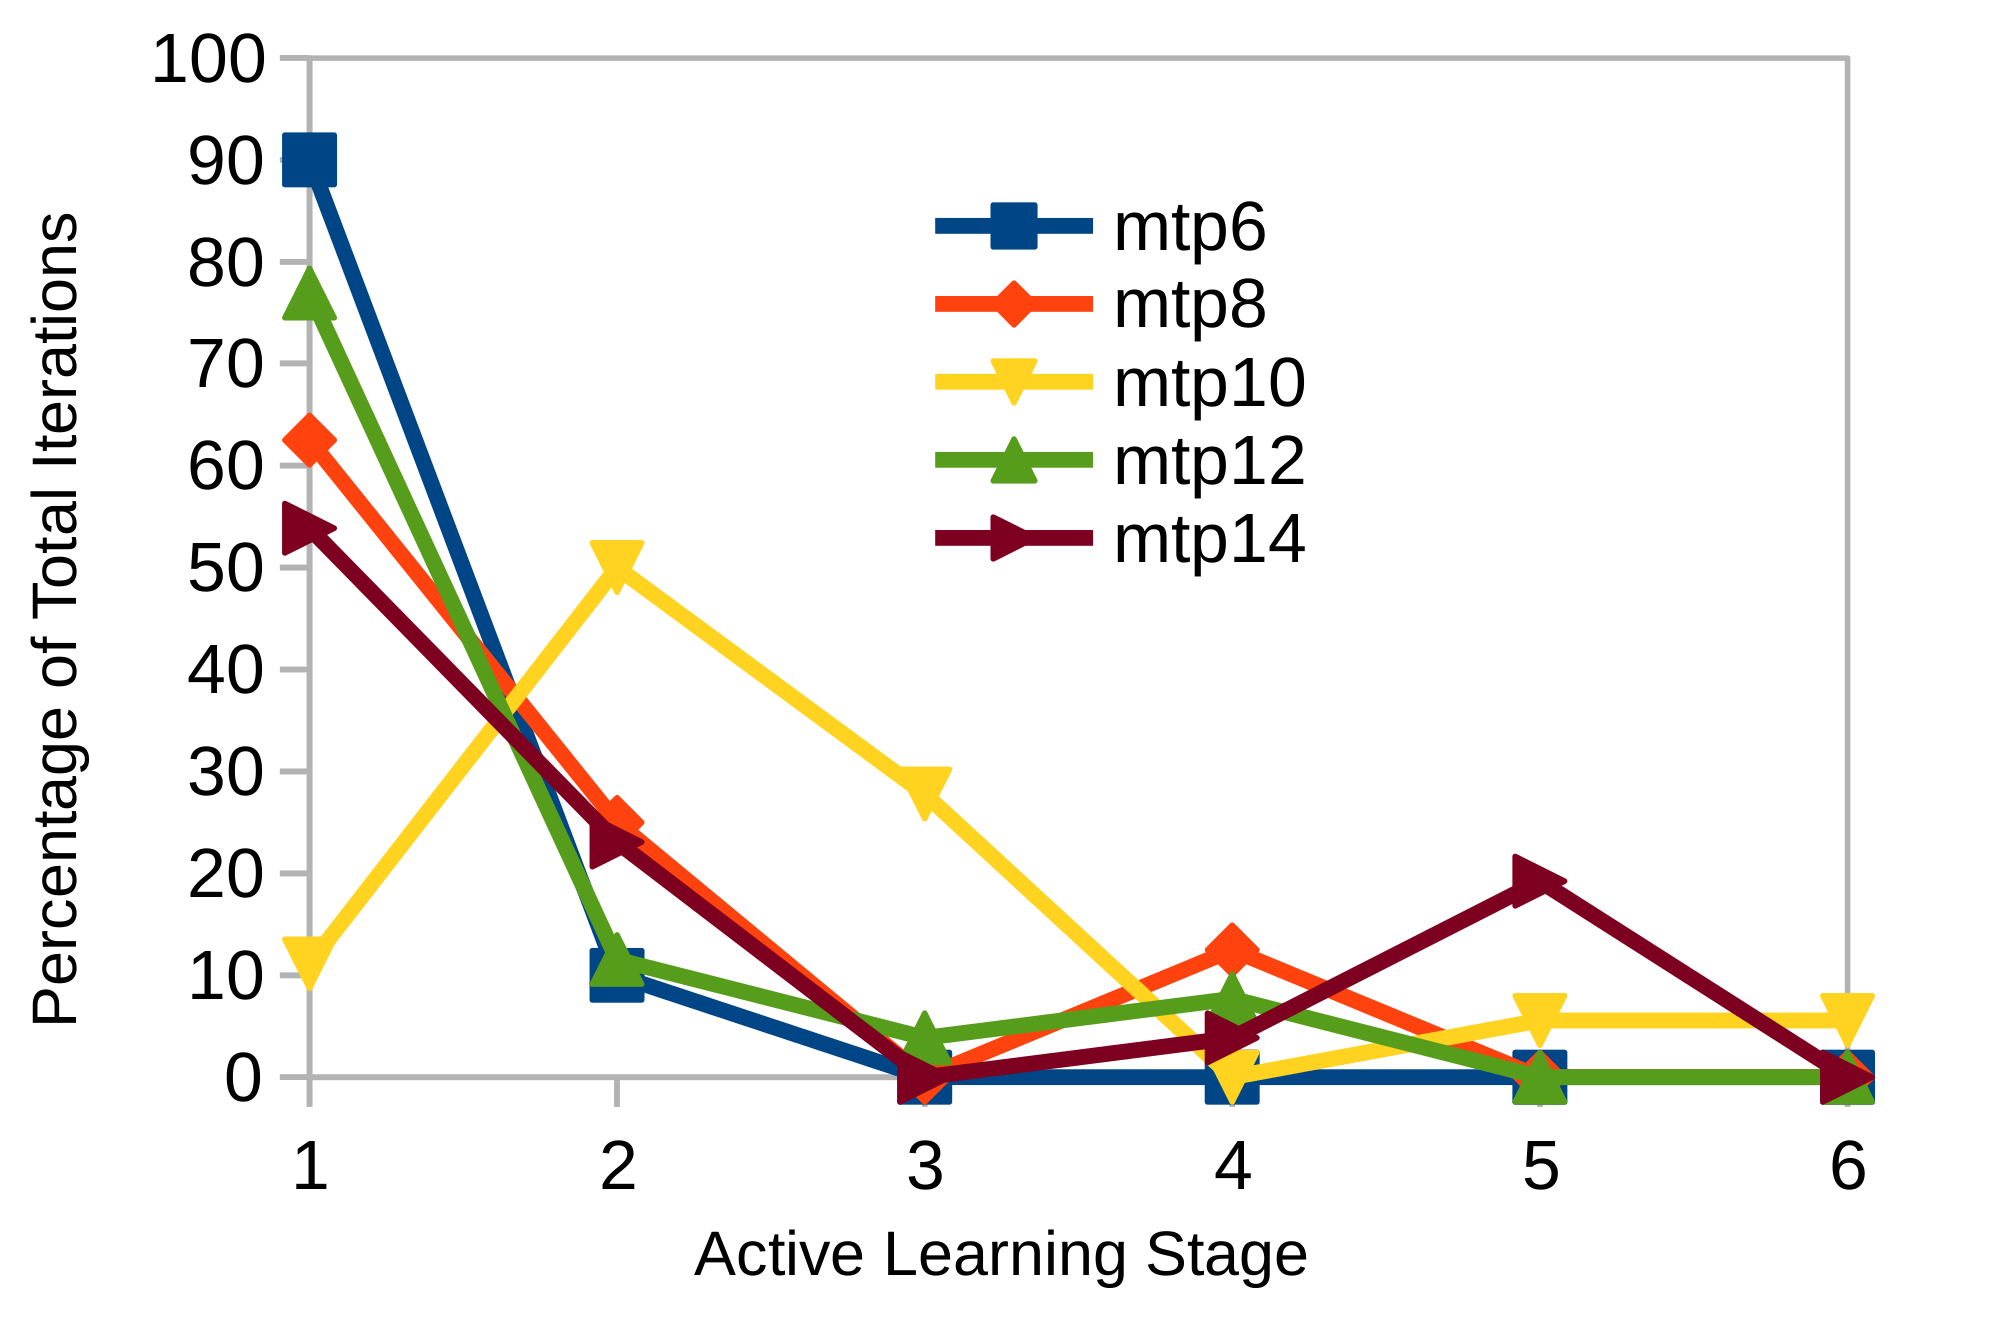
\includegraphics[width=\linewidth]{assets/iterations.png}
  \caption{Percentage of iterations spent at each stage}
  \label{fig:iterations}
\end{figure}

All of the MTPs, except MTP10 which is likely an outlier, learn the majority of the interactions needed in the first two stages of the training scheme. From a point of view this suggests that the active learning representation, the bottom-up approach is valid, reaching the representation that generates no preselected configurations—the same result that occurs when an MTP is directly trained on some of the latter stages. From a practical view, MTP directly trained on later levels resulted in a slightly lower count of total iterations, although the computational expense is considerably higher and the performance is not much different. In the cases where the MTPs spent a larger percentage of their total iterations in prior stages, stages 3 and 6 tended to offer limited additional benefits; comparatively, stages 4 and 5 tended to give some additional learning. However, this observation is fairly expected, given that the longest dimension of stages 3 and 6 is approximately twice the cutoff radius used. However, due to the lack of a larger sample pool, is it difficult to determine the training scheme's effectiveness with more certainty. 

Figure \ref{fig:levels} shows the total number of training configurations obtained through an entire active learning run. Generally, MTPs can be expected to select more configurations with increasing levels, although we note that MTP 6 has more training configurations than MTP 8. The exact relationship is uncertain due to the sample size of active learning runs we managed to perform. This relationship may also vary based on the scenario of the MTP and the training scheme used. 

\begin{figure}[ht]
  \centering
  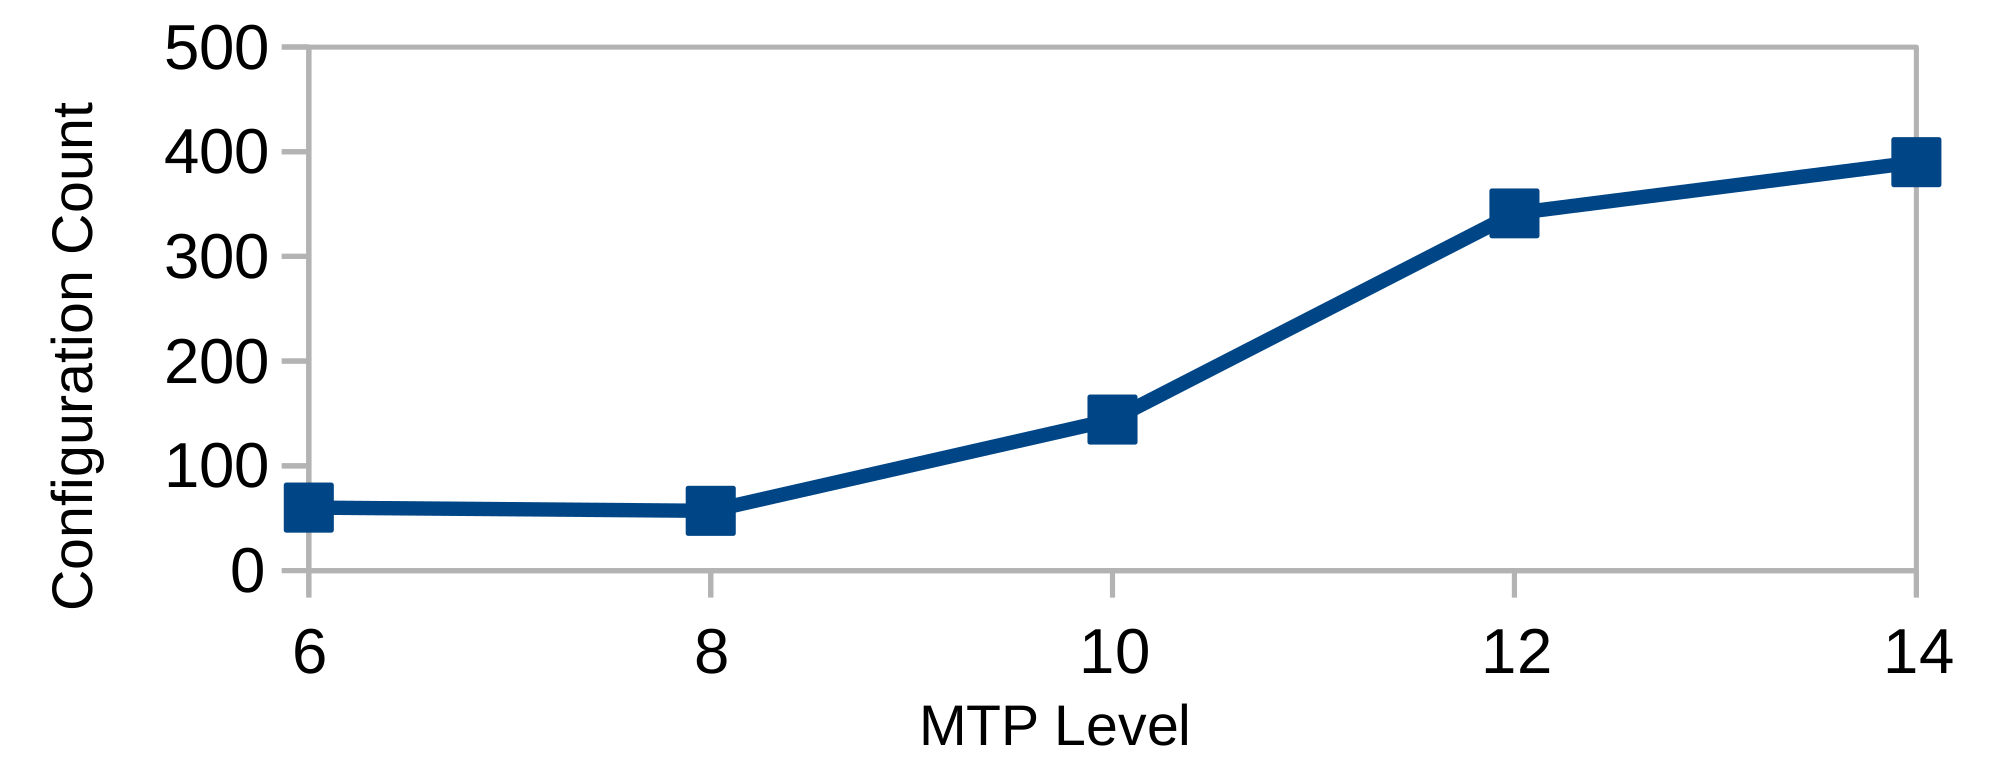
\includegraphics[width=\linewidth]{assets/levels.png}
  \caption{Number of the iterations }
  \label{fig:levels}
\end{figure}

To explore the effect of the initial parameters on the MTPs training, we prepare an ensemble of 30 MTPs per level. With the training sets generated by the active learning runs, we train MTPs, each with random initial parameters. Recording the average training energy and force errors on a per-atom basis for each of the MTPs, we generate Figure \ref{fig:errors}. 

\begin{figure}[ht]
  \centering
  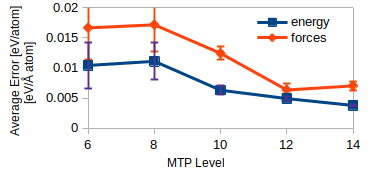
\includegraphics[width=\linewidth]{assets/errors.png}
  \caption{Average training errors. 30 training runs, 95\% confidence interval.}
  \label{fig:errors}
\end{figure}

As expected, the average training errors for force and energy decrease with the level of the MTP. We also find that for a given training dataset per level of MTP, the variance of the initial parameters affects the training errors more for lower MTP levels, and for force errors more than energy errors which are reasonable as force is the derivative of energy. 

\subsection{Solid Potassium Validation}
To validate the results of the ensembles of trained MTP for elastic properties, energy calculations of BCC lattices near the baseline lattice parameter are prepared for each MTP. The resultant plot is available in Figure \ref{fig:elastic}.

\begin{figure}[ht]
  \centering
  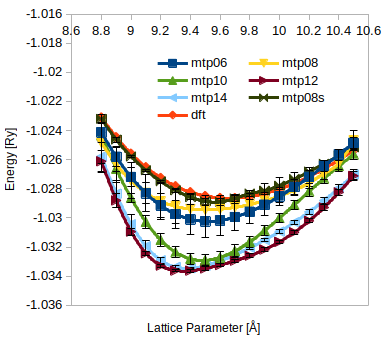
\includegraphics[width=\linewidth]{assets/curve.png}
  \caption{Elastic curve predictions. General purpose MTPs, DFT reference, and specialized MTP (08s). 95\% confidence interval.}
  \label{fig:elastic}
\end{figure}

We generally find fairly poor accuracy when trying to predict the elastic curve using the general-purpose MTPs of all levels. Interestingly, it appears that the predictions are not necessarily better for MTPs of higher levels, with MTP 8 performing the best out of all the levels. One possibility is overfitting, as suggested by the less symmetrical and irregular elastic curves produced by the MTPs of higher levels although we suspect that the issue may lie with the training sets for the available levels of MTPs. Since the initial training sets are closely representative of the elastic curve and are consistent between all the MTPs, the MTPs with a smaller number would have a higher proportion of their training data related to the elastic curve, giving a better representation. However, the levels of MTPs being examined are not particularly high, and higher MTP levels around 20 may provide better predictions. To further illustrate this we utilize active learning on MTP08, the best performer, with a training scheme specialized for solid data, yielding a near-perfect agreement with the DFT reference. Using, a $2^{nd}$ order Birch fit, Table \ref{tab:elastic} shows the predicted values of the general MTP of level 8 and one trained on specialized data. 

\begin{table}[htbp]
  \centering
  \caption{\bf Elastic }
  \begin{tabular}{cccc}
  \hline
  Property & DFT &  MTP08 & MTP08\\ 
  \hline
  Lattice Parameter [Å] & 5.11 & 5.04 & 5.12\\
  Bulk Modulus [GPa]& 3.9 & 3.3 & 3.8\\
  Equilibirum Volume [Å$^3$]& 66.72 & 64.02 & 67.33\\
  \hline
  \end{tabular}
  \label{tab:elastic}
\end{table}

We find that the MTP gives overall good performance for most cases although its predictions of very specific properties that rely on precise prediction in a narrow range of conditions may be lacking for the MTP level examined. This limitation is especially true for MTPs which span diverse representations like different phases, and we find that lower-level MTPs can still provide good predictions when specifically trained. However, the MTP levels being examined are still relatively low, and higher levels may lead to a richer representation. In cases where specific conditions are of interest, we would strongly recommend performing active learning on training scenarios adapted to the conditions or experiencing with significantly higher MTP levels.

\subsection{Liquid Potassium Predictions}
To assess the validity of the MTP for property prediction in the liquid phase, we rely on radial distribution function (RDF) prediction. Due to the lack of quantum mechanical reference liquid potassium data in the literature, we perform our own \textit{ab initio} (DFT-based) MD runs. To generate this reference benchmark, we took an arbitrary 54-atom iteration from one of the previously discarded active learning runs as an initial frame to an \textit{ab initio} run at 600K. Due to the computational expense and limited time scope of the project, only 0.01 ps of the simulation were available for RDF calculation. Combined with the relatively small simulation cell, the reference data is noisy and certain peaks are exaggerated. Next for each MTP ensemble, the MTP with the lowest training error from each ensemble was subject to an NVT starting from a BCC simulation cell of 16000 atoms at 600K. Figure \ref{fig:rdf} shows the resultant RDFs.

\begin{figure}[ht]
  \centering
  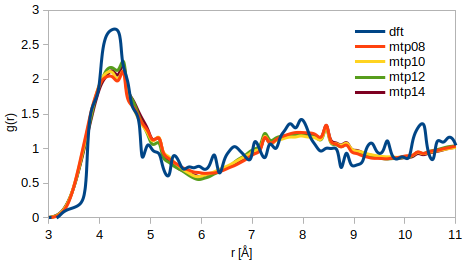
\includegraphics[width=\linewidth]{assets/rdf.png}
  \caption{Elastic curve predictions. General purpose MTPs, DFT reference, and specialized MTP (08s). 95\% confidence interval.}
  \label{fig:rdf}
\end{figure}

Overall, the MTPs examined are all within excellent agreement with each other except for MTP6 which was not stable in the larger simulations, losing atoms. Within the limited quality of the \textit{ab initio} data, we would also agree that there appears to be a good agreement between the predictions and the reference. The spikes, especially those at a radius of approximately 4.5 Å, have softened as the simulation has progressed and the liquid potassium atoms shift further from their initial positions. We expect an excellent match given sufficient computation.

\subsection{Configurational Errors}
Having examined the MTP's performance in prediction tasks, we consider it's 


% \section{Corresponding author}

% We require manuscripts to identify a single corresponding author. The corresponding author typically is the person who submits the manuscript and handles correspondence throughout the peer review and publication process. If other statements about author contribution and contact are needed, they can be added in addition to the corresponding author designation.

% %Example with the corresponding author designated by an asterisk:

% %\author{Author One\authormark{1} and Author Two\authormark{2,*}}

% %\address{\authormark{1}Peer Review, Publications Department,
% %Optica Publishing Group, 2010 Massachusetts Avenue NW,
% %Washington, DC 20036, USA\\
% %\authormark{2}Publications Department, Optica Publishing Group,
% %2010 Massachusetts Avenue NW, Washington, DC 20036, USA\\
% %%\authormark{3}xyz@optica.org}

% %\email{\authormark{*}xyz@optica.org}}

% %Example with the corresponding author designated by an asterisk and a note indicating equal contributions by two authors.

% %\author{Author One\authormark{1,3} and Author %Two\authormark{2,3,*}}

% %\address{\authormark{1}Peer Review, Publications Department,
% %Optica Publishing Group, 2010 Massachusetts Avenue NW, %Washington, DC 20036, USA\\
% %\authormark{2}Publications Department, Optica Publishing Group, %2010 Massachusetts Avenue NW, Washington, DC 20036, USA\\
% %\authormark{3}The authors contributed equally to this work.\\
% %\authormark{*}xyz@optica.org}}

% %\section{Examples of Article Components}
% %\label{sec:examples}

% The sections below show examples of different article components.

% \section{Figures and Tables}

% Do not place figures and tables at the back of the manuscript. Figures and tables should be placed and sized as they are likely to appear in the final article. 

% Figures and Tables should be labelled and referenced in the standard way using the \verb|\label{}| and \verb|\ref{}| commands.

% \subsection{Sample Figure}

% Figure \ref{fig:false-color} shows an example figure.

% \begin{figure}[ht]
% \centering
% \fbox{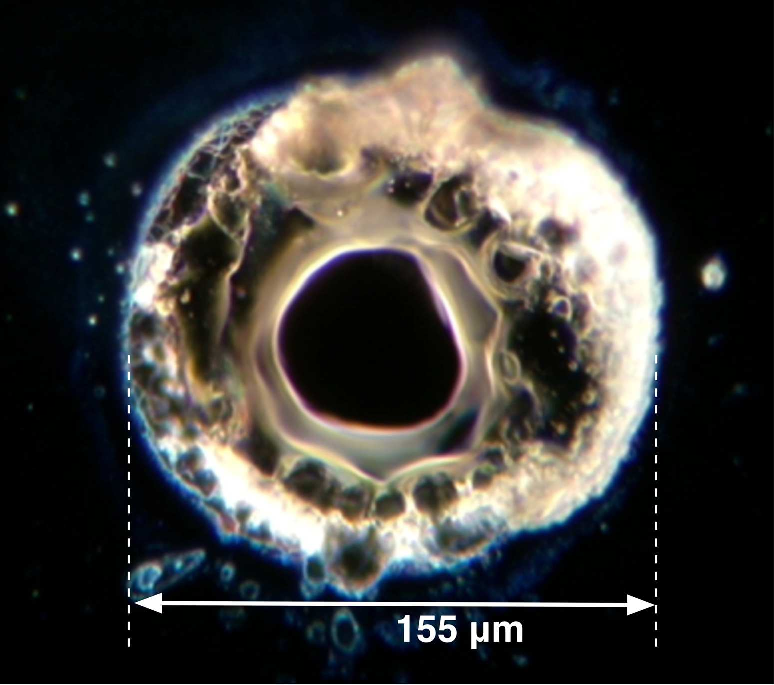
\includegraphics[width=\linewidth]{opticafig1}}
% \caption{Dark-field image of a point absorber.}
% \label{fig:false-color}
% \end{figure}

% \subsection{Sample Table}

% Table \ref{tab:shape-functions} shows an example table.

% \begin{table}[htbp]
% \centering
% \caption{\bf Shape Functions for Quadratic Line Elements}
% \begin{tabular}{ccc}
% \hline
% local node & $\{N\}_m$ & $\{\Phi_i\}_m$ $(i=x,y,z)$ \\
% \hline
% $m = 1$ & $L_1(2L_1-1)$ & $\Phi_{i1}$ \\
% $m = 2$ & $L_2(2L_2-1)$ & $\Phi_{i2}$ \\
% $m = 3$ & $L_3=4L_1L_2$ & $\Phi_{i3}$ \\
% \hline
% \end{tabular}
%   \label{tab:shape-functions}
% \end{table}

% \section{Sample Equation}

% Let $X_1, X_2, \ldots, X_n$ be a sequence of independent and identically distributed random variables with $\text{E}[X_i] = \mu$ and $\text{Var}[X_i] = \sigma^2 < \infty$, and let
% \begin{equation}
% S_n = \frac{X_1 + X_2 + \cdots + X_n}{n}
%       = \frac{1}{n}\sum_{i}^{n} X_i
% \label{eq:refname1}
% \end{equation}
% denote their mean. Then as $n$ approaches infinity, the random variables $\sqrt{n}(S_n - \mu)$ converge in distribution to a normal $\mathcal{N}(0, \sigma^2)$.

% \section{Sample Algorithm}

% Algorithms can be included using the commands as shown in algorithm \ref{alg:euclid}.

% \begin{algorithm}
% \caption{Euclid’s algorithm}\label{alg:euclid}
% \begin{algorithmic}[1]
% \Procedure{Euclid}{$a,b$}\Comment{The g.c.d. of a and b}
% \State $r\gets a\bmod b$
% \While{$r\not=0$}\Comment{We have the answer if r is 0}
% \State $a\gets b$
% \State $b\gets r$
% \State $r\gets a\bmod b$
% \EndWhile\label{euclidendwhile}
% \State \textbf{return} $b$\Comment{The gcd is b}
% \EndProcedure
% \end{algorithmic}
% \end{algorithm}

% \subsection{Supplementary materials in Optica Publishing Group journals}
% Optica Publishing Group journals allow authors to include supplementary materials as integral parts of a manuscript. Such materials are subject to peer-review procedures along with the rest of the paper and should be uploaded and described using the Prism manuscript system. Please refer to the \href{https://opg.optica.org/submit/style/supplementary_materials.cfm}{Author Guidelines for Supplementary Materials in Optica Publishing Group Journals} for more detailed instructions on labeling supplementary materials and your manuscript. For preprints submitted to Optica Open a link to supplemental material should be included in the submission, but do not upload the material.

% \textbf{Authors may also include Supplemental Documents} (PDF documents with expanded descriptions or methods) with the primary manuscript. At this time, supplemental PDF files are not accepted for JOCN or PRJ. To reference the supplementary document, the statement ``See Supplement 1 for supporting content.'' should appear at the bottom of the manuscript (above the References heading). Supplemental documents are not accepted for Optica Open preprints.

% \begin{figure}[ht!]
% \centering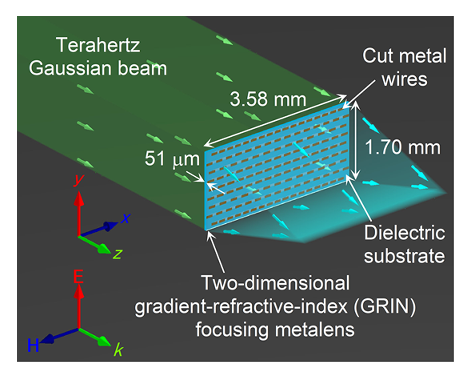
\includegraphics{opticafig2}
% \caption{Terahertz focusing metalens.}
% \end{figure}


% \subsection{Sample Dataset Citation}

% 1. M. Partridge, "Spectra evolution during coating," figshare (2014), http://dx.doi.org/10.6084/m9.figshare.1004612.

% \subsection{Sample Code Citation}

% 2. C. Rivers, "Epipy: Python tools for epidemiology," Figshare (2014) [retrieved 13 May 2015], http://dx.doi.org/10.6084/m9.figshare.1005064.

% \section{Backmatter}
% Backmatter sections should be listed in the order Funding/Acknowledgment/Disclosures/Data Availability Statement/Supplemental Document section. An example of backmatter with each of these sections included is shown below.

% \begin{backmatter}
% \bmsection{Funding} Content in the funding section will be generated entirely from details submitted to Prism. Authors may add placeholder text in the manuscript to assess length, but any text added to this section in the manuscript will be replaced during production and will display official funder names along with any grant numbers provided. If additional details about a funder are required, they may be added to the Acknowledgments, even if this duplicates information in the funding section. See the example below in Acknowledgements. For preprint submissions, please include funder names and grant numbers in the manuscript.

% \bmsection{Acknowledgments} The section title should not follow the numbering scheme of the body of the paper. Additional information crediting individuals who contributed to the work being reported, clarifying who received funding from a particular source, or other information that does not fit the criteria for the funding block may also be included; for example, ``K. Flockhart thanks the National Science Foundation for help identifying collaborators for this work.''

% \bmsection{Disclosures} Disclosures should be listed in a separate section at the end of the manuscript. List the Disclosures codes identified on the \href{https://opg.optica.org/submit/review/conflicts-interest-policy.cfm}{Conflict of Interest policy page}. If there are no disclosures, then list ``The authors declare no conflicts of interest.''

% \smallskip

% \noindent Here are examples of disclosures:


% \bmsection{Disclosures} ABC: 123 Corporation (I,E,P), DEF: 456 Corporation (R,S). GHI: 789 Corporation (C).

% \bmsection{Disclosures} The authors declare no conflicts of interest.


% \bmsection{Data Availability Statement} A Data Availability Statement (DAS) will be required for all submissions beginning 1 March 2021. The DAS should be an unnumbered separate section titled ``Data Availability'' that
% immediately follows the Disclosures section. See the \href{https://opg.optica.org/submit/review/data-availability-policy.cfm}{Data Availability Statement policy page} for more information.

% There are four common (sometimes overlapping) situations that authors should use as guidance. These are provided as minimal models, and authors should feel free to
% include any additional details that may be relevant.



% \begin{enumerate}
% \item When datasets are included as integral supplementary material in the paper, they must be declared (e.g., as "Dataset 1" following our current supplementary materials policy) and cited in the DAS, and should appear in the references.

% \bmsection{Data availability} Data underlying the results presented in this paper are available in Dataset 1, Ref. [3].

% \item When datasets are cited but not submitted as integral supplementary material, they must be cited in the DAS and should appear in the references.

% \bmsection{Data availability} Data underlying the results presented in this paper are available in Ref. [3].

% \item If the data generated or analyzed as part of the research are not publicly available, that should be stated. Authors are encouraged to explain why (e.g.~the data may be restricted for privacy reasons), and how the data might be obtained or accessed in the future.

% \bmsection{Data availability} Data underlying the results presented in this paper are not publicly available at this time but may be obtained from the authors upon reasonable request.

% \item If no data were generated or analyzed in the presented research, that should be stated.

% \bmsection{Data availability} No data were generated or analyzed in the presented research.
% \end{enumerate}

% \bigskip

% \noindent Data availability statements are not required for preprint submissions.

% \bmsection{Supplemental document}
% See Supplement 1 for supporting content. 

% \end{backmatter}

% \section{References}

% Note that \emph{Optics Letters} and \emph{Optica} short articles use an abbreviated reference style. Citations to journal articles should omit the article title and final page number; this abbreviated reference style is produced automatically when the \emph{Optics Letters} journal option is selected in the template, if you are using a .bib file for your references.

% However, full references (to aid the editor and reviewers) must be included as well on a fifth informational page that will not count against page length; again this will be produced automatically if you are using a .bib file.

% \bigskip
% \noindent Add citations manually or use BibTeX. See \cite{Zhang:14,OPTICA,FORSTER2007,testthesis,manga_rao_single_2007}.

% Bibliography
\bibliography{sample}

% Full bibliography added automatically for Optics Letters submissions; the following line will simply be ignored if submitting to other journals.
% Note that this extra page will not count against page length
\bibliographyfullrefs{sample}

%Manual citation list
%\begin{thebibliography}{1}
%\bibitem{Zhang:14}
%Y.~Zhang, S.~Qiao, L.~Sun, Q.~W. Shi, W.~Huang, %L.~Li, and Z.~Yang,
 % \enquote{Photoinduced active terahertz metamaterials with nanostructured
  %vanadium dioxide film deposited by sol-gel method,} Opt. Express \textbf{22},
  %11070--11078 (2014).
%\end{thebibliography}

% Please include bios and photos of all authors for aop articles
\ifthenelse{\equal{\journalref}{aop}}{%
\section*{Author Biographies}
\begingroup
\setlength\intextsep{0pt}
\begin{minipage}[t][6.3cm][t]{1.0\textwidth} % Adjust height [6.3cm] as required for separation of bio photos.
  \begin{wrapfigure}{L}{0.25\textwidth}
    \includegraphics[width=0.25\textwidth]{john_smith.eps}
  \end{wrapfigure}
  \noindent
  {\bfseries John Smith} received his BSc (Mathematics) in 2000 from The University of Maryland. His research interests include lasers and optics.
\end{minipage}
\begin{minipage}{1.0\textwidth}
  \begin{wrapfigure}{L}{0.25\textwidth}
    \includegraphics[width=0.25\textwidth]{alice_smith.eps}
  \end{wrapfigure}
  \noindent
  {\bfseries Alice Smith} also received her BSc (Mathematics) in 2000 from The University of Maryland. Her research interests also include lasers and optics.
\end{minipage}
\endgroup
}{}


\end{document}
